\chapter{Gestión de Proyectos}

Scrum es un marco de gestión de proyectos para el desarrollo incremental de productos, valiéndose de equipos autoorganizados. 



\subsection{Proyecto Scrum}

Un proyecto, en ingeniería de software, es un esfuerzo temporal que se lleva a cabo para crear un sistema, software o resultado único\footnote{Se parafrasea la definición del PMBOOK \cite{PMBOK-2004}.}. Los proyectos son organizados, en una empresa u organización, por el proceso de administración de proyectos. Según este proceso, el ciclo de vida de los proyectos se puede dividir en tres fases: inicio, ejecución y cierre (ver figura \ref{fig:PMIProject}). En la administración de proyectos es necesario planificar los proyectos y dicha actividad se suele hacer en la fase de inicio ("Starting phase" o "Project Start"). Pero, a diferencia de la metodología clásica (ver figura \ref{fig:PMIProject}) en que la planificación estaba siempre al inicio y el desarrollo en la fase de ejecución, en el marco Scrum la planificación se distribuye durante todo el ciclo de vida del proyecto y en la fase de ejecución se hace el desarrollo incremental de productos (por incrementos de producto) en iteraciones cortas (Sprint) donde cada iteración tiene su respectiva planificación (ver figura \ref{fig:ScrumProject}) y su incremento de producto, en caso de haberlo logrado.

\begin{figure}[h]
  \centering
  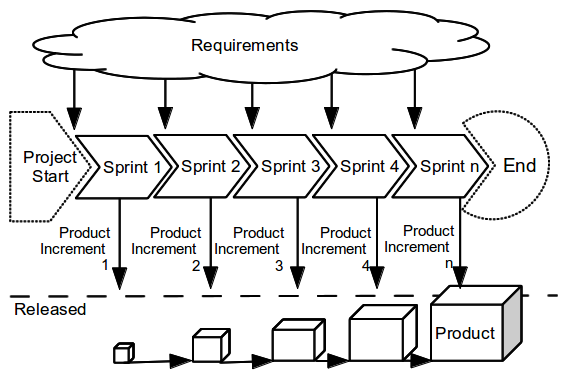
\includegraphics[width=0.90\textwidth]{ScrumProject}
  \caption{Proyecto Scrum}
  \centering
  \label{fig:ScrumProject} %\ref{fig:ScrumProject}
\end{figure}

Entonces podemos decir que en Scrum se piensa en muchos planes periódicos (a corto plazo). Los mismo pueden estar en un plan mayor a largo plazo pero de carácter flexible. También se puede realizar un plan global de entregables en base a los incrementos de producto estimado. Pero, desde esta perspectiva, hay que considerar que aunque se trabaje con planificaciones, los planes no son contratos a respetar a rajatabla.

%Triangle of Project Management
\subsection{Triángulo de la Gestión de proyectos}

El marco de Scrum cambia el triángulo clásico de la gestión de proyectos. El compromiso ya no es entre el tiempo, presupuesto y calidad; sino que se basa en el triángulo de: Presupuesto (Costo), Tiempo y funcionalidad (alcance) (ver figura \ref{fig:ScrumProjectManagementTriangle}). Además, tradicionalmente se ha intentado fijar el alcance para negociar y variar el presupuesto y el tiempo. En cambio, desde la agilidad, se intenta mantener fijos el tiempo y el presupuesto mientras se varía el alcance \cite{Martin-Alaimo-2014}.

\begin{figure}[h]
  \centering
  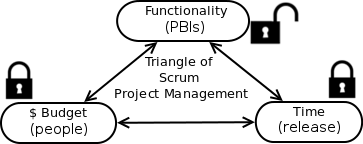
\includegraphics[width=0.80\textwidth]{ScrumProjectManagementTriangle}
  \caption{Triángulo de Gestión de Proyectos Scrum}
  \centering
  \label{fig:ScrumProjectManagementTriangle} %\ref{fig:ScrumProjectManagementTriangle}
\end{figure}

\subsection{Planificación de entregables}

Con esta metodología tampoco es necesario hacer una entrega final (o "releasing") ya que se pueden hacer entregas paulatinas. Para hacer entregas intermedias se puede crear un plan de muy alto nivel para múltiples Sprints durante una planificación de lanzamiento. Este plan de entregables o de de lanzamientos es una guía con la que se pretende reflejar las expectativas sobre las qué funciones se implementarán y cuando se completarán \cite{Scrum-Institute-2015}. También sirve como una base para monitorear el progreso dentro del proyecto. Pero siempre hay que considerar que no es un plan equivalente a un plan clásico, los ítos de releases no deberían ser compromisos rígidos y contractuales, y el desarrollo del proyecto no debería centrarse en respetar el plan. Por este motivo el plan de lanzamiento no es un plan estático. Pues, se cambia durante todo el proyecto cuando nuevos requerimientos o conocimientos están disponible y, por ejemplo, cuando entradas en el Scrum Product Backlog cambian y re-estiman. Por lo tanto este plan debe ser revisado y actualizado en intervalos regulares, por ejemplo, después de cada Sprint.

Para crear un plan de entregables se deben tener disponibles las siguientes cosas:

\begin{enumerate}
\item Un Product Backlog priorizado y estimado.
\item La velocidad estimada del Equipo Scrum.
\item Las condiciones de satisfacción (metas para la agenda, el alcance, los recursos)
\end{enumerate}

\subsection{Métricas}

Las métricas son una combinación de atributos cuantificables pertinentes que comunican información relevante acerca de la calidad de nuestros productos y nuestra productividad\footnote{\cite{INCOSE-2005}}. Para la ingeniería del software, las métricas proporcionan una indicación de la calidad de algún tipo de representación del software basadas en un conjunto de medidas indirectas\footnote{\cite{Roger-Pressman-2002}}. O sea que las mismas están relacionadas a unidades de medida e indicadores que ayudan a medir, descubrir y tomar decisiones para mejorar, corregir problemas, hacer estimaciones, controlar calidad, evaluar productividad y hacer control de proyectos. Intentar medir para mejorar nuestra comprensión de entidades particulares es tan poderoso en ciencia, en ingeniería de software como en cualquier disciplina.

Bajo el marco Scrum ayuda al equipo a medir su propio desempeño para poder hacer cambios basados en hechos. También es un soporte a la gestión de proyectos para poder medir el avance del proyecto, revisar la productividad, el desempeño\footnote{Las métricas se pueden usar para medir desempeño, pero no se deben utilizar en forma punitiva ni tampoco en sistemas de evaluacion de desempeño de empleados.} del equipo y poder hacer comparaciones relativas entre evolución de diferentes equipos. 

\subsubsection{Unidades de medida}

Para poder usar métricas y medir es necesario unidades de medida. Las más usadas son:

\begin{enumerate}

\item {\textbf{Story Points:}
El Story Points o SP es una unidad de medida que indica una cantidad de alcanse o trabajo que puede ser entregado o tamaño de producto estimado para entregar. Es una unidad de medida que representa la complejidad o esfuerzo necesario para terminar las tareas de una historia \footnote{\cite{Jipson-Thomas-2015}}. El SP sirve como estimación de la complejidad en forma relativa y sumativa que hacen los desarrolladores. También hay que tener en cuenta que es una unidad subjetiva que depende de qué equipo hace la estimación de medida.
}

\item {\textbf{Business Value Point:}
El Business Value o BV es el valor añadido que la historia aporta al negocio\footnote{\cite{Pointet-Botton-2012}}. A semejanza del SP, el Business Value Point o BVP sirve como estimación del valor de negocio en forma relativa y sumativa que hace el PO. También hay que tener en cuenta que es una unidad subjetiva que depende de qué PO o equipo de personas hace la estimación de medida.
}

\end{enumerate}

\subsubsection{Indicadores}

Hay muchos indicadores que nos pueden ser de utilidad, como por ejemplo los siguientes\footnote{Scott y Jeff \cite{Scott-Jeff-2013} y la  Scrumalliance en un artículo llamado "Velocity, How to Calculate and Use Velocity to Help Your Team and Your Projects", por Catia Oliveira (6 February 2014).}:

\begin{enumerate}

\item {\textbf{Velocity:} La 'velocidad'\footnote{"Sum of original estimates of all accepted work" \cite{Scott-Jeff-2013}.} es el número de unidades de trabajo o puntos de historia SP estimados y aceptados por un equipo en una iteración Sprint. En otras palabras, es el conjunto de puntos de historia totales conseguidos (aceptados) por el equipo al final de cada Sprint\footnote{\cite{Jipson-Thomas-2015}}.}

Esta definición es la clásica y es algo genérica. Hay tres formas más específicas de interpretar y medir la velocidad:

  \begin{enumerate}

  \item{\textbf{Velocidad de trabajo:} cuando la velocidad muestra la cantidad de trabajo o funcionalidad que un equipo entrega (aceptada) en un sprint\footnote{"Velocidad en la que el equipo pueda completar el trabajo en un Sprint, número de funcionalidades entregadas en un sólo Sprint o Número de Story Points hecho en un determinado Sprint" \cite{SBOK-2013}}, incluyendo las de valor indirecto. En este sentido las historia de usuario completadas (tomadas del backlog técnico) que tienen valor indirecto para el cliente, las correcciones de errores, deuda técnica, migraciones y refactorizaciones sí cuentan en la velocidad. En este caso, la velocidad del equipo da pocas indicaciones sobre el verdadero valor de negocio entregado y más sobre la capacidad que puede producir. Pues la velocidad, en este sentido, no suele tener relación directa con el valor de negocio entregado. Como no se suele aclarar bien la definición de velocidad se suele entender que se trata de esta perspectiva pero, sin embargo, en Scrum clásico se sobreentiende que los equipos deben entregar valor de punta a punta, por lo que la velocidad debería estar ligada al valor como la siguiente definición.
  }

  \item{\textbf{Velocity en nueva funcionalidad:} cuando la velocidad muestra solo la cantidad de funcionalidad de valor para el negocio que un equipo entrega (aceptada) en un sprint. En este sentido las historia de usuario que no tienen ningún valor para el cliente o incompletas, las correcciones de errores y las refactorizaciones no cuentan en la velocidad\footnote{\cite{David-Koontz-2014}}. En este caso, la velocidad del equipo da un indicio sobre el valor de negocio entregado por el equipo. En Scrum original o clásico se sobreentiende que las historias son las que aportan valor, por tal motivo a veces no se aclara explícitamente esto.
  }
  
  \item{\textbf{Value Velocity:} es una forma interesante para medir la productividad (sugerida por James Shore\footnote{\cite{James-Shore-2015}}) similar a la velocidad tradicional o velocidad de trabajo, excepto que se basa en estimaciones de valor de negocio (Business Value Point) hechas por el PO antes de la planeación.
  }
  
  \end{enumerate}

\item {\textbf{Average Velocity:} De la valocity de cada Sprint se calcula la velocidad promedio o "Average Velocity" que es el número de unidades de trabajo o SP promedio estimados y aceptados por un equipo en un conjunto de iteraciones Sprint. En un equipo ágil de velocidad estable, la velocidad promedio (por ejemplo de los últimos 4 Sprints) es un indicador adelantado de la velocidad estimada para el próximo Sprint (bajo las mismas condiciones de los Sprints usados para calcularla).}

\item {\textbf{Work Capacity:} La Capacidad es la suma de todos los trabajos reportados durante el Sprint, esten terminados o no\footnote{Scott y Jeff \cite{Scott-Jeff-2013}}. La capacidad es generalmente igual o superior a la Velocity. Aunque la Capacidad puede, en raras ocasiones, caer por debajo de la velocidad. Esto se debe a que la velocidad se calcula en base a las estimaciones originales de trabajo, mientras que la capacidad se calcula en base a la suma de trabajo real reportado\footnote{Scott y Jeff \cite{Scott-Jeff-2013}}. Por lo que en el caso de que esto suceda, lo que indica es que el equipo ha sobre estimando la complejidad de los trabajos solicitados. También existen otras formas de calcular o entender la capacidad. Por ejemplo:

  \begin{enumerate}
  
  \item {\textbf{Capacidad en puntos ideales:} La capacidad puede ser una idealización basada en la velocidad promedio, o sea, los puntos de la historia que se pueden considerar gastar en la próxima carrera de velocidad.\footnote{\cite{Satish-Thatte-2013}}}

  \item {\textbf{Capacidad en horas:} La capacidad puede ser calculada en horas basados en la cantidad de miembros y la cantidad de horas efectivas de trabajo en un Sprint. Por ejemplo en un equipo de 8 miembros, con 6 horas de trabajo efectivo y un Sprint de 10 días, la capacidad en horas es igual a 480 hs (8 x 6 hs x 10).}

  \end{enumerate}

Cuando se definió el marco de trabajo, como algo mínimo de cosas para que funcione, se dejó lo más simple posible. Debido a ello, el concepto de Velocity sí es partes del marco de trabajo, pero Working capacity no lo es, aunque es ampliamente usado \footnote{Erich Buhler, Agilib.org 2015, Proyecto Mercury 2015 (LAN), \cite{Erich-Buhler-Coach-2015}.}.
}

\item {\textbf{Focus Factor:} El factor de foco revela el foco que el equipo ha tenido para entregar valor y su prestancia. El mismo es la relación entre la Velocity y la capacidad de trabajo: ( Velocity / Work Capacity ) x 100\%. La misma debe permanecer en la vecindad de 80 \% en promedio para un equipo saludable. Estos puntos de datos por debajo del 80 por ciento indican un equipo que está interrumpido o incapaz de convertir su trabajo estimado en trabajo aceptado mostrando poca previcibilidad. Cuando el valor es alto, cercano al 100, el equipo ha estado bajo la previsión de su capacidad, aunque esto no indica necesariamente que están trabajando bien. Por ejemplo, el equipo puede estar aparentando ser perfecto forzando la coincidencia.}

\item {\textbf{Targeted Value Increase (TVI+)} El TVI+ responde a cuánto cambio ha habido en la velocidad del equipo a través del tiempo desde el primer Sprint. Es la Velocity del Sprint actual dividido la Velocity Original (velocity del primer sprint): ( Current Sprint’s Velocity / Original Velocity ) x 100\%. Sirve para medir el aumento de la contribución de valor de un equipo en base a su velocidad origen Sprint a Sprint.
Por ejemplo, si el resultado es 200\% significa que el equipo ha duplicado su capacidad de resolver con éxito la complejidad requerida.
}

%Otras: Percentage of Adopted Work, Percentage of Found Work, Accuracy of Estimation, Accuracy of Forecast, Targeted Value Increase (TVI+), Success at Scale

\item {\textbf{Business Value Delivered:}
Un indicador relevante es el valor de negocio entregado. Se pueden contabilizar los BV entregados en cada Sprint.
}

\item {\textbf{Happiness Metric:}
Un estudio de Harvard muestra que la felicidad aumenta la producción de cualquier tipo de trabajo, pues "la gente feliz es 12 \% más productiva"\footnote{\cite{U-K-University-2014}}. Además, un principio de la agilidad es desarrollar en torno a individuos motivados. En base a esto podemos intentar medir la felicidad Sprint a Sprint\footnote{\cite{Jeff-2014}}. 

La felicidad del equipo es un indicativo de la salud del equipo en relación a su capacidad de entrega de valor. Para medir la felicidad del equipo podemos hacer encuestas o responder las siguientes preguntas:

  \begin{enumerate}
  \item {¿Cómo me siento acerca de mi trabajo? Se puede usar una escala de 1 a 5 (ver figura \ref{fig:HappinessMetric}). 
  
  \begin{figure}[h]
  \centering
  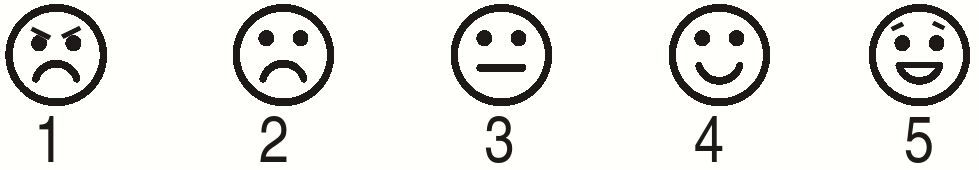
\includegraphics[width=0.40\textwidth]{HappinessMetric}
  \caption{Medida de satisfacción}
  \centering
  \label{fig:HappinessMetric} %\ref{fig:HappinessMetric}
\end{figure}

  Otra escala para medir felicidad puede ser de siete puntos. Por ejemplo a la pregunta... ¿Cómo calificaría su felicidad en este momento? Se puede responder con 1 que es totalmente triste, 2 es muy triste , 3 es triste, 4 es ni feliz ni triste, 5 es bastante feliz, 6 es muy feliz y 7 es completamente feliz\footnote{\cite{U-K-University-2014}}.
  }
  
  \item {¿Qué va a hacer que me sienta mejor?}
  \end{enumerate}

Cuando tenemos la información de cada miembro del equipo, el equipo puede hacer una lluvia de ideas de cómo hacer para mejorar y aumentar la felicidad en el siguiente Sprint y darle curso y seguimiento a las acciones propuestas.

También se puede medir la felicidad de los Stakeholder como indicador de grado de satisfacción que indica qué tan contentos estuvieron con los resultados del Sprint y con la Review. Este relevamiento relacionado a la persepción de valor entregado se puede hacer en la misma Review.

}


\end{enumerate}


Por último, hay que tener en cuenta que para que las métricas estén bajo un marco Scrum deben respetar los principios de la agilidad. La medida principal es el software funcionando. Las métricas deben ser un medio de comunicación efectiva e impulsar la transparencia. Deben servir al equipo para que se auto-organize en procesos de corrección de desvíos y mojora contínua, apoyando la reflexión sobre cómo ser más efectivos. Y, principalmente, se debe buscar siempre la simplicidad. Las métricas que agregan complejidad innecesaria o sobre-información no son acordes a la agilidad.
